\chapter{Sampling Distributions and the Central Limit Theorem}\index{central limit theorem}\index{sampling distribution}

A national poll asks about 1,000 people a question and then announces what more than
150 million voters think, ``plus or minus 3 percentage points.'' How can 1,000 people
possibly speak for 150 million? And where does that 3 come from?

The answer is one of the most surprising facts in all of mathematics. Averages
behave far more predictably than the individual values they come from. Take almost
any population, as lopsided and strange as you like, draw a large random sample, and
compute its average. If you did that over and over, the averages would pile up in a
bell-shaped normal curve, every time. That fact is the \newterm{Central Limit Theorem}
(CLT), and it is the reason every confidence interval and significance test in the
chapters that follow works.

\section{Statistics Vary from Sample to Sample}
A \newterm{parameter} is a number that describes a whole population, like the true
average watch time $\mu$ of every video on a streaming site. A \newterm{statistic} is a
number computed from a sample, like the average $\bar{x}$ of 30 randomly chosen videos.
We use statistics to estimate parameters, because measuring a whole population is
usually impossible.

Draw a different random sample, and you get a different $\bar{x}$. This is
\newterm{sampling variability}, and it is not a mistake: it is what random samples do.
The key question is \emph{how much} a statistic varies. To answer it, imagine taking
every possible sample of the same size and computing the statistic for each. The
distribution of all those values is the statistic's \newterm{sampling distribution}.

Nobody can take every possible sample. But a computer can take ten thousand, which is
close enough to see the pattern.

\section{A Simulation}\index{central limit theorem!simulation}
On a video site, most videos are watched for only a few minutes, but a few are watched
for an hour. Suppose watch times follow a strongly skewed distribution with mean
$\mu = 10$ minutes and standard deviation $\sigma = 10$ minutes. (The program uses the
exponential distribution from the Poisson and Exponential chapter, which has exactly
that shape.) For each sample size $n = 1$, $5$, and $30$, the program draws 10,000
random samples, averages each one, and draws a histogram of the 10,000 averages:

\begin{minted}{python}
import numpy as np
import matplotlib.pyplot as plt
from scipy.stats import norm

rng = np.random.default_rng(1)
MEAN = 10            # average watch time, in minutes
SAMPLES = 10_000     # how many samples we draw for each size

fig, axes = plt.subplots(1, 3, figsize=(10, 3))
for ax, n in zip(axes, [1, 5, 30]):
    # 10,000 samples of n watch times each; average each sample
    data = rng.exponential(MEAN, size=(SAMPLES, n))
    means = data.mean(axis=1)
    print(f"n = {n:2}: mean of x-bar = {means.mean():.2f}, "
          f"sd of x-bar = {means.std():.2f}, theory = {MEAN / np.sqrt(n):.2f}")

    ax.hist(means, bins=50, density=True, color="#005892")
    x = np.linspace(0, means.max(), 300)
    ax.plot(x, norm.pdf(x, MEAN, MEAN / np.sqrt(n)), color="orange")
    ax.set_title(f"sample size n = {n}")
    ax.set_xlabel("sample mean (minutes)")
fig.tight_layout()
fig.savefig("clt_simulation.png")
\end{minted}
\begin{verbatim}
n =  1: mean of x-bar = 10.01, sd of x-bar = 10.00, theory = 10.00
n =  5: mean of x-bar = 9.96, sd of x-bar = 4.43, theory = 4.47
n = 30: mean of x-bar = 9.96, sd of x-bar = 1.82, theory = 1.83
\end{verbatim}

\begin{figure}[H]
\centering
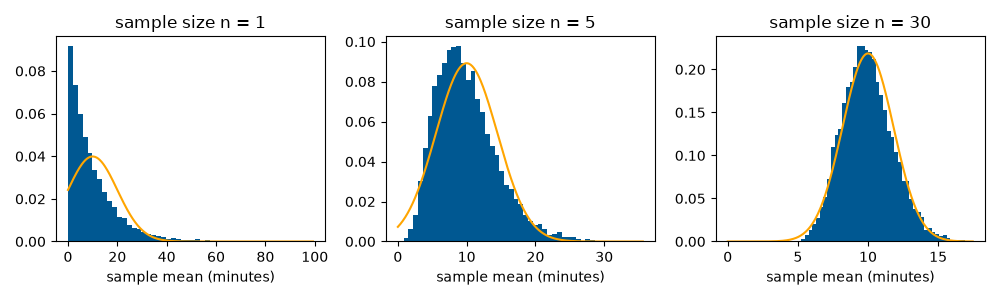
\includegraphics[width=\textwidth]{clt_simulation.png}
\caption{Histograms of 10,000 sample means for samples of size 1, 5, and 30, drawn
from a skewed population. The orange curve is the normal distribution the CLT predicts.}
\label{fig:clt-simulation}
\end{figure}

Three things happen as $n$ grows, and they are the whole story of this chapter:
\begin{enumerate}
\item \textbf{Center:} the sample means are always centered at the population mean, 10.
\item \textbf{Spread:} they cluster more tightly, with a standard deviation that matches
$\frac{10}{\sqrt{n}}$.
\item \textbf{Shape:} they become normal. With $n = 1$, the histogram is just the skewed
population. With $n = 5$, it is still lopsided. With $n = 30$, it fits the normal curve
almost perfectly, even though no individual watch time is anywhere near normal.
\end{enumerate}

\section{The Center and Spread of $\bar{x}$}
The first two facts follow from the rules in the Random Variables chapter. Think of a
sample as $n$ independent random variables $X_1, \dots, X_n$, each with mean $\mu$ and
standard deviation $\sigma$. Then $\bar{x} = \frac{1}{n}(X_1 + \cdots + X_n)$, and
\begin{itemize}
\item by linearity, $E[\bar{x}] = \frac{1}{n}(\mu + \cdots + \mu) = \frac{1}{n}(n\mu) = \mu$;
\item because variances of independent variables add, the sum has variance $n\sigma^2$,
and dividing by $n$ divides the variance by $n^2$:
$\operatorname{Var}(\bar{x}) = \frac{n\sigma^2}{n^2} = \frac{\sigma^2}{n}$.
\end{itemize}

\begin{mdframed}[style = important, frametitle = {Mean and Standard Deviation of $\bar{x}$}]
For random samples of size $n$ from a population with mean $\mu$ and standard deviation $\sigma$,
$$\mu_{\bar{x}} = \mu, \qquad \sigma_{\bar{x}} = \frac{\sigma}{\sqrt{n}}$$
\end{mdframed}

Because $\mu_{\bar{x}} = \mu$, we say $\bar{x}$ is an \newterm{unbiased} estimator: it does
not tend to guess too high or too low. The formula $\frac{\sigma}{\sqrt{n}}$ has a
sobering consequence, the \newterm{square-root law}: to cut the spread in half, you need
four times as many observations. To make an estimate 10 times more precise, you need
100 times the data. This is the same $\frac{1}{\sqrt{n}}$ you saw in the Monte Carlo
Simulation chapter, and it is the same reason.

\section{The Central Limit Theorem}
The third fact, about shape, is the deep one.

\begin{mdframed}[style = important, frametitle = {The Central Limit Theorem}]
When $n$ is large, the sampling distribution of $\bar{x}$ is approximately normal, with
mean $\mu$ and standard deviation $\frac{\sigma}{\sqrt{n}}$, no matter what shape the
population has.
\end{mdframed}

How large is ``large''? It depends on the population. If the population is itself
normal, $\bar{x}$ is exactly normal for every $n$. If it is roughly symmetric, $n = 10$ or
so is plenty. If it is strongly skewed, you need more. The common AP rule of thumb is
$n \geq 30$, which is why the Statistical Inferences for Means chapter accepts $n \geq 30$
as a way to satisfy its ``normal or large sample'' condition.

The CLT also explains why so many things in nature are close to normal. A person's
height is the sum of many small effects from many genes and from nutrition. A
measurement error is the sum of many small disturbances. Sums of many small,
independent pieces are approximately normal, whatever the pieces look like.

\textbf{Example}: An elevator sign says ``Maximum 12 people or 1,000 kg.'' Adult weights
have mean 80 kg and standard deviation 15 kg. If 12 randomly chosen adults get on, what
is the chance they exceed 1,000 kg?

\textbf{Solution}: Twelve people exceed 1,000 kg exactly when their average weight
exceeds $\frac{1000}{12} \approx 83.3$ kg. By the CLT, $\bar{x}$ is approximately normal with
mean 80 and standard deviation $\frac{15}{\sqrt{12}} \approx 4.33$. So
$$z = \frac{83.3 - 80}{4.33} \approx 0.77, \qquad P(\bar{x} > 83.3) = P(Z > 0.77) \approx 0.22$$
More than a one-in-five chance. That is why real elevators are built to carry far more than
the posted limit.

Notice how differently individuals and averages behave. The chance that one random adult
weighs more than 95 kg is $P(Z > 1) \approx 0.16$. The chance that the \emph{average} of 4
adults is more than 95 kg is $P\left(Z > \frac{95 - 80}{15/\sqrt{4}}\right) = P(Z > 2) \approx 0.023$,
about seven times less likely. Averages are hard to push to extremes.

\section{The Sampling Distribution of a Proportion}\index{sample proportion}
A sample proportion $\hat{p}$ (``p-hat'') is secretly a mean. Code each person as 1 for
``yes'' and 0 for ``no.'' Then $\hat{p}$ is the average of those 0s and 1s, and the
count of yeses, $X = n\hat{p}$, is binomial (from the Binomial and Geometric Distributions
chapter). Dividing the binomial mean $np$ and standard deviation $\sqrt{np(1-p)}$ by $n$:

\begin{mdframed}[style = important, frametitle = {Mean and Standard Deviation of $\hat{p}$}]
$$\mu_{\hat{p}} = p, \qquad \sigma_{\hat{p}} = \sqrt{\frac{p(1-p)}{n}}$$
The sampling distribution of $\hat{p}$ is approximately normal when $np \geq 10$ and $n(1-p) \geq 10$.
\end{mdframed}

That last line is the CLT for 0/1 data, and it is the \textbf{large counts} condition you
will check before every confidence interval for a proportion in the next chapter.

Now we can answer the opening question. For a poll of $n = 1000$ with $p$ near $0.5$,
$\sigma_{\hat{p}} = \sqrt{\frac{0.5 \cdot 0.5}{1000}} \approx 0.0158$. About 95\% of a normal
distribution lies within 2 standard deviations of the center, and $2(0.0158) \approx 0.03$:
the famous ``plus or minus 3 points.'' Notice that the population size, 150 million, appears
nowhere in the formula. A well-drawn random sample of 1,000 is just as accurate for a whole
country as for a single large city.

\textbf{Example}: A candidate truly has 55\% support. What is the chance that a random poll
shows them losing ($\hat{p} < 0.5$)?

\begin{minted}{python}
import numpy as np

rng = np.random.default_rng(2)
p = 0.55             # true support for the candidate

for n in [100, 1000]:
    # 10,000 polls of n voters; p-hat is the fraction who say yes
    p_hat = rng.binomial(n, p, size=10_000) / n
    wrong = np.mean(p_hat < 0.5)
    print(f"n = {n:4}: mean {p_hat.mean():.3f}, sd {p_hat.std():.4f}, "
          f"polls showing a loss: {wrong:.4f}")
\end{minted}
\begin{verbatim}
n =  100: mean 0.550, sd 0.0496, polls showing a loss: 0.1338
n = 1000: mean 0.550, sd 0.0158, polls showing a loss: 0.0005
\end{verbatim}
With 100 voters, about 13\% of polls get the winner wrong. With 1,000, only about 1 in
2,000 do. The normal model agrees well for $n = 1000$, where
$P\left(Z < \frac{0.5 - 0.55}{0.0157}\right) = P(Z < -3.18) \approx 0.0007$. For $n = 100$, it
gives $0.157$, while the exact binomial answer is $0.135$. The gap comes from $\hat{p}$
moving in steps of 0.01 with only 100 voters, so a smooth curve is a rougher fit. Larger
samples make the normal approximation better.

\begin{Exercise}[title={Center and Spread}, label=clt_basic]
A population has mean 50 and standard deviation 12. You take random samples of size 36.
\begin{enumerate}
\item What are the mean and standard deviation of the sampling distribution of $\bar{x}$?
\item Find $P(\bar{x} > 53)$.
\item How large a sample would make $\sigma_{\bar{x}}$ at most 1?
\end{enumerate}
\end{Exercise}
\begin{Answer}[ref=clt_basic]
\begin{enumerate}
\item $\mu_{\bar{x}} = 50$ and $\sigma_{\bar{x}} = \frac{12}{\sqrt{36}} = 2$.
\item $z = \frac{53 - 50}{2} = 1.5$, so $P(\bar{x} > 53) = P(Z > 1.5) \approx 0.067$.
\item $\frac{12}{\sqrt{n}} \leq 1$ means $\sqrt{n} \geq 12$, so $n \geq 144$.
\end{enumerate}
\end{Answer}

\begin{Exercise}[title={Watch Times}, label=clt_video]
Watch times on the video site have mean 10 minutes and standard deviation 10 minutes, and
are strongly skewed. For a random sample of 40 videos, estimate the probability that the
average watch time is more than 12 minutes. Why is it reasonable to use a normal model
even though watch times are not normal?
\end{Exercise}
\begin{Answer}[ref=clt_video]
$\sigma_{\bar{x}} = \frac{10}{\sqrt{40}} \approx 1.58$, so $z = \frac{12 - 10}{1.58} \approx 1.26$ and
$P(\bar{x} > 12) \approx P(Z > 1.26) \approx 0.10$. The normal model is reasonable because of the
CLT: $n = 40$ is large enough that the sample mean is approximately normal even though the
population is skewed. (The exact answer for this population is about 0.107, so the
approximation is close.)
\end{Answer}

\begin{Exercise}[title={True or False?}, label=clt_misconception]
A student says, ``The Central Limit Theorem says that if I take a big enough sample, my
data will be normally distributed.'' Is that right? Explain.
\end{Exercise}
\begin{Answer}[ref=clt_misconception]
No. A bigger sample makes the \emph{data} look more like the population, so a sample of
watch times stays skewed no matter how large it is. The CLT is about the
\emph{sampling distribution of the mean}: if you took many samples and averaged each one,
those averages would be approximately normal.
\end{Answer}

\begin{Exercise}[title={Dice Averages}, label=clt_dice]
Change \filename{clt\_simulation.py} so that each observation is a roll of a fair die,
using \mintinline{python}{rng.integers(1, 7, size=(SAMPLES, n))}, and use sample sizes 1, 2,
and 10. Describe the three histograms. (For one die, $\mu = 3.5$ and $\sigma \approx 1.71$.)
\end{Exercise}
\begin{Answer}[ref=clt_dice]
With $n = 1$, the histogram is flat: six equal bars. With $n = 2$, it is a triangle peaking
at 3.5, the shape of the dice sums from the Discrete Probability chapter. With $n = 10$, it is
already close to a bell curve centered at 3.5 with standard deviation about
$\frac{1.71}{\sqrt{10}} \approx 0.54$. A flat, symmetric population needs only a small $n$ for
the CLT to kick in.
\end{Answer}
